%%%%%%%%%%%%%%%%%%%%%%%%%%%%%%%%%%%%%%%%%%%%%%%%%%%%%%%%%%%%%%%%%%%%%%%%%%%%%%%%
%	Latex Notes Template
%	Zach Neveu
%	zachary.neveu@gmail.com
%%%%%%%%%%%%%%%%%%%%%%%%%%%%%%%%%%%%%%%%%%%%%%%%%%%%%%%%%%%%%%%%%%%%%%%%%%%%%%%%

% Geometry, font
\documentclass[12pt, letter]{article}
\usepackage[margin=0.8in]{geometry}
\usepackage[T1]{fontenc}
\usepackage{fourier}
\usepackage{titling}
\setlength{\droptitle}{-5em} 
\usepackage[parfill]{parskip}
\usepackage{graphicx}
\graphicspath{{imgs/}}
\usepackage{hyperref}
\usepackage{booktabs}


% Math stuff
\usepackage{amssymb}
\usepackage{amsmath}
\usepackage{bm}

%acronyms
\usepackage{acronym}
\newacro{FIR}{finite impulse response}

% Code Highlighting
\usepackage{minted}
\usemintedstyle{solarizedlight}

\author{Zach Neveu}
\title{ Homework 3: Optimization of FIR Filter Design }

\begin{document}
\maketitle

\subsection*{Designs}
For this homework, 12 different HLS designs for an FIR filter were synthesized. These designs all contain variations of loop unrolling, loop fission, changing memory type, datatype optimization, and changing position of control flow in loops. The full list of experiments run is shown in Table \ref{tab:experiments}.

\begin{table}[h]
	\centering
	\caption{List of Experiments and Descriptions}
	\label{tab:experiments}
	\begin{tabular}{lrrrrr}
	\toprule
	Design 				& Data/Coeffs. Bit Width  & Unroll Factor & Fission & BRAM Ports & Control in Loop \\
	\midrule
	basic				& 10 & 1 & 0 & 0 & 1 \\
	\midrule
	fission				& 10 & 1 & 1 & 0 & 0 \\
	\midrule
	remove\_if			& 10 & 1 & 0 & 0 & 0 \\
	\midrule
	unroll\_2			& 10 & 2 & 1 & 0 & 0\\
	\midrule
	unroll\_all			& 10 & 11 & 1 & 0 & 0\\
	\midrule
	unroll\_all\_2pbram	& 10 & 11 & 1 & 2 & 0\\
	\midrule
	basic\_1pbram		& 10 & 1 & 1 & 1 & 1\\
	\midrule
	unroll\_all\_1pbram	& 10 & 11 & 1 & 1 & 0\\
	\midrule
	32b\_unroll\_all	& 32 & 11 & 1 & 0 & 0\\
	\midrule
	32b\_unroll\_2		& 32 & 2 & 1 & 0 & 0\\
	\midrule
	32b\_fission		& 32 & 1 & 1 & 0 & 0\\
	\midrule
	32b\_basic			& 32 & 1 & 0 & 0 & 1\\
	\bottomrule
	\end{tabular}
\end{table}

\subsection*{Results}
Latency and Area were calculated for each synthesized filter design. For the purposes of this report, area was calculated according to formula \ref{eq:area}. Latency and Area were then compared using a Pareto plot which can be seen in \ref{fig:pareto}.

\begin{equation}
	Area = 100*BRAM+100*DSP+MAX(FF, LUT)
	\label{eq:area}
\end{equation}

\begin{figure}[h]
	\centering
	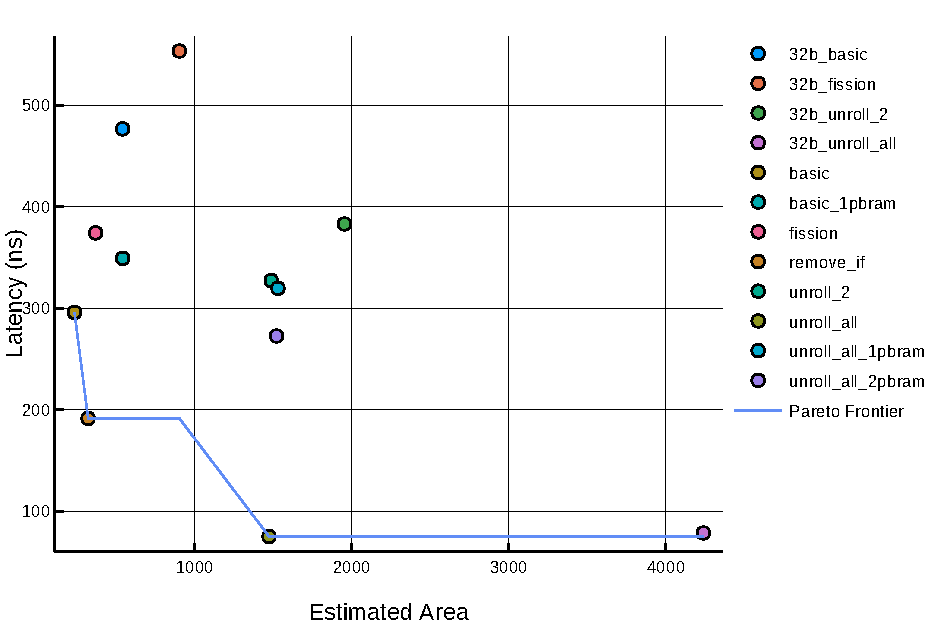
\includegraphics[width=0.8\textwidth]{pareto.pdf}
	\caption{Pareto Chart of Designs}
	\label{fig:pareto}
\end{figure}

\subsection*{Discussion}
The lowest latency design was \texttt{unroll\_all} with \texttt{unroll\_all\_2pbram} as a close second. This shows that unrolling loops can seriously improve latency when necessary. The lowest area design was \texttt{basic}. Only one other point, \texttt{remove\_if} appears on the Pareto frontier. This design uses negligibly more resources than \texttt{basic}, and decreases latency by more than $30\%$, so this design, in my opinion, is the best trade-off between area and latency. Based on these results, it appears that removing control flow from loops, and unrolling loops provide the largest performance trade-offs. While loop unrolling requires significantly more resources, removing control flow from loops comes at almost no cost. Finally, the cost of using non-optimized data types is quite significant. No 32 bit designs appear on the Pareto frontier and most lie quite far from it.


\end{document}
